\section{Effets :}
\emph{Interface :}

L'utilisateur choisit un effet parmi la liste d'effets affichée en bas de l'écran, ce qui affiche les 
réglages disponibles (s'il y en a). L'utilisateur peut ensuite choisir de confirmer ou d'annuler la modification
apportée par l'effet choisi.
\\

\emph{Structure du code :}

Les effets sont rassemblés dans le package filters (fr.ubordeaux.pimp.filters).
La classe \emph{Retouching} contient les réglages de luminosité, contraste, saturation et teinte.
La classe \emph{Convolution} contient tous les effets liés à la convolution (flou, détection de contour etc.).
Toutes ces méthodes sont appelées lors de l'appui de boutons ou de glissement de seekbars. Les seekbars ont généralement
une étendue allant de 0 à 255 (sauf pour les réglages de teinte), et certains effets nécessitent des valeurs pouvant être
négatives. Ainsi la valeur de seekbar est modifiée dans la méthode appelante de ces mêmes effets.
\subsection{Luminosité (Brightness) :}
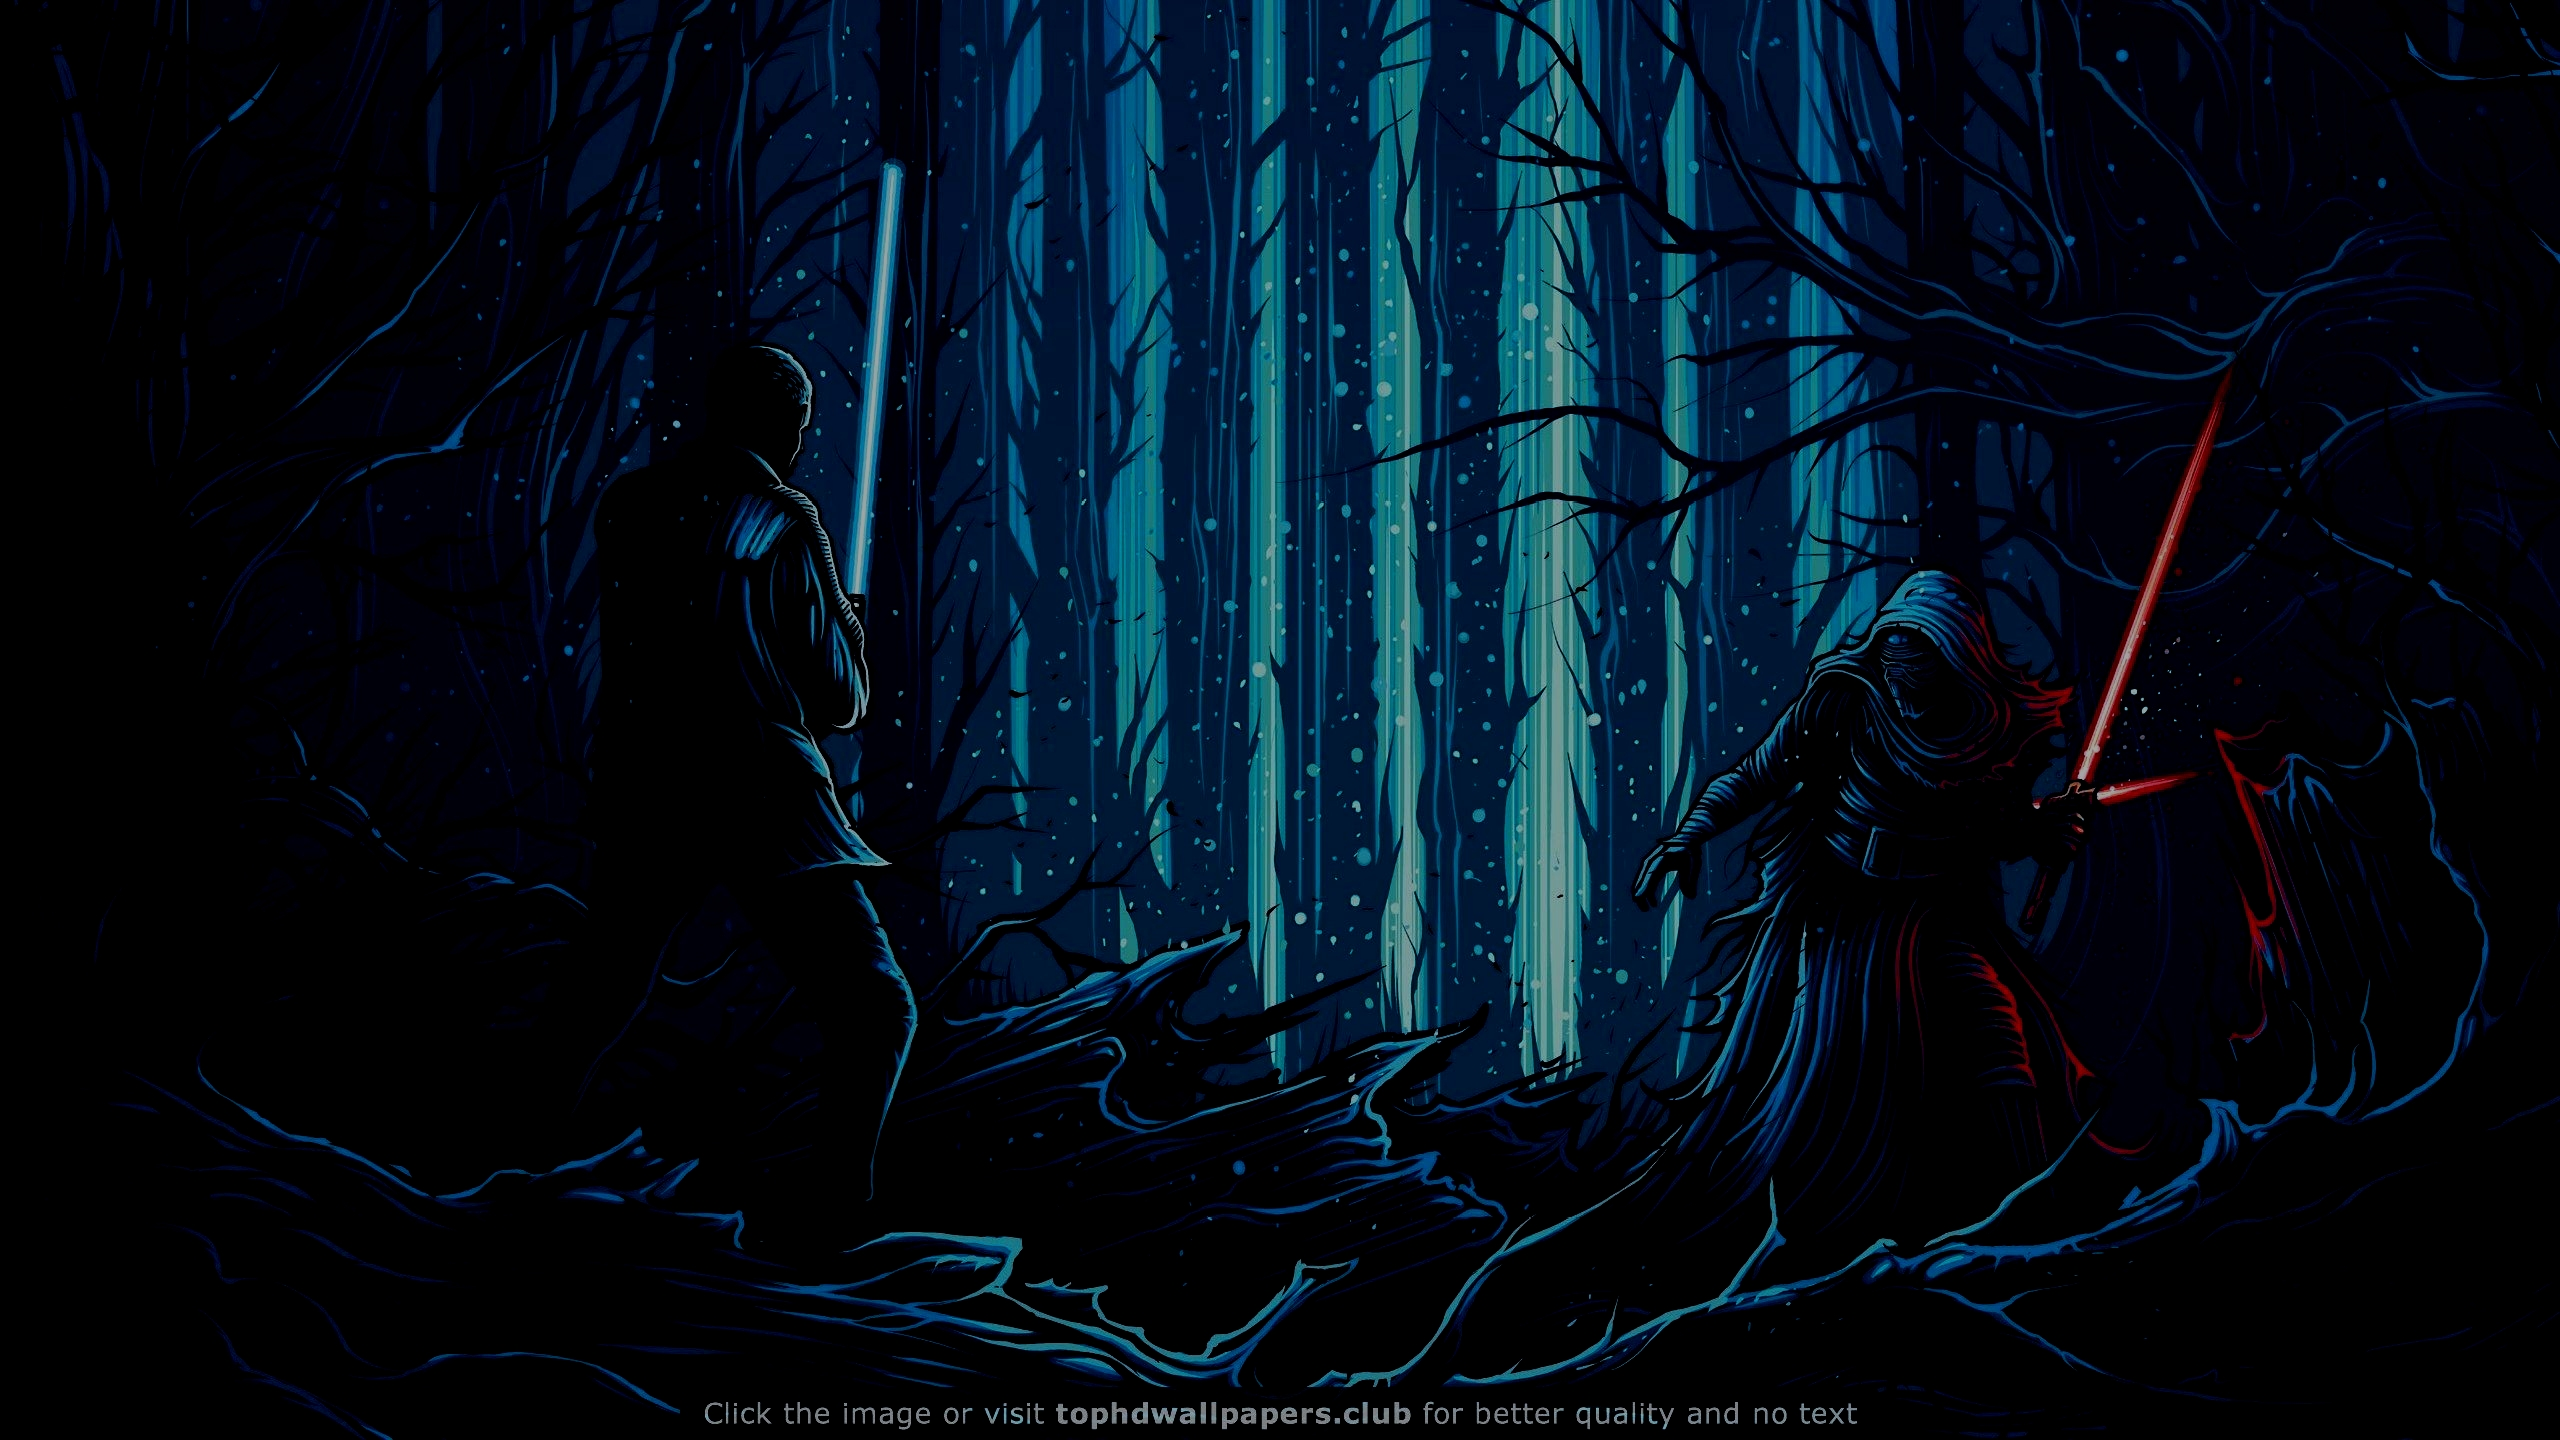
\includegraphics[width=0.5\textwidth]{report_src/brightness_low.jpeg}
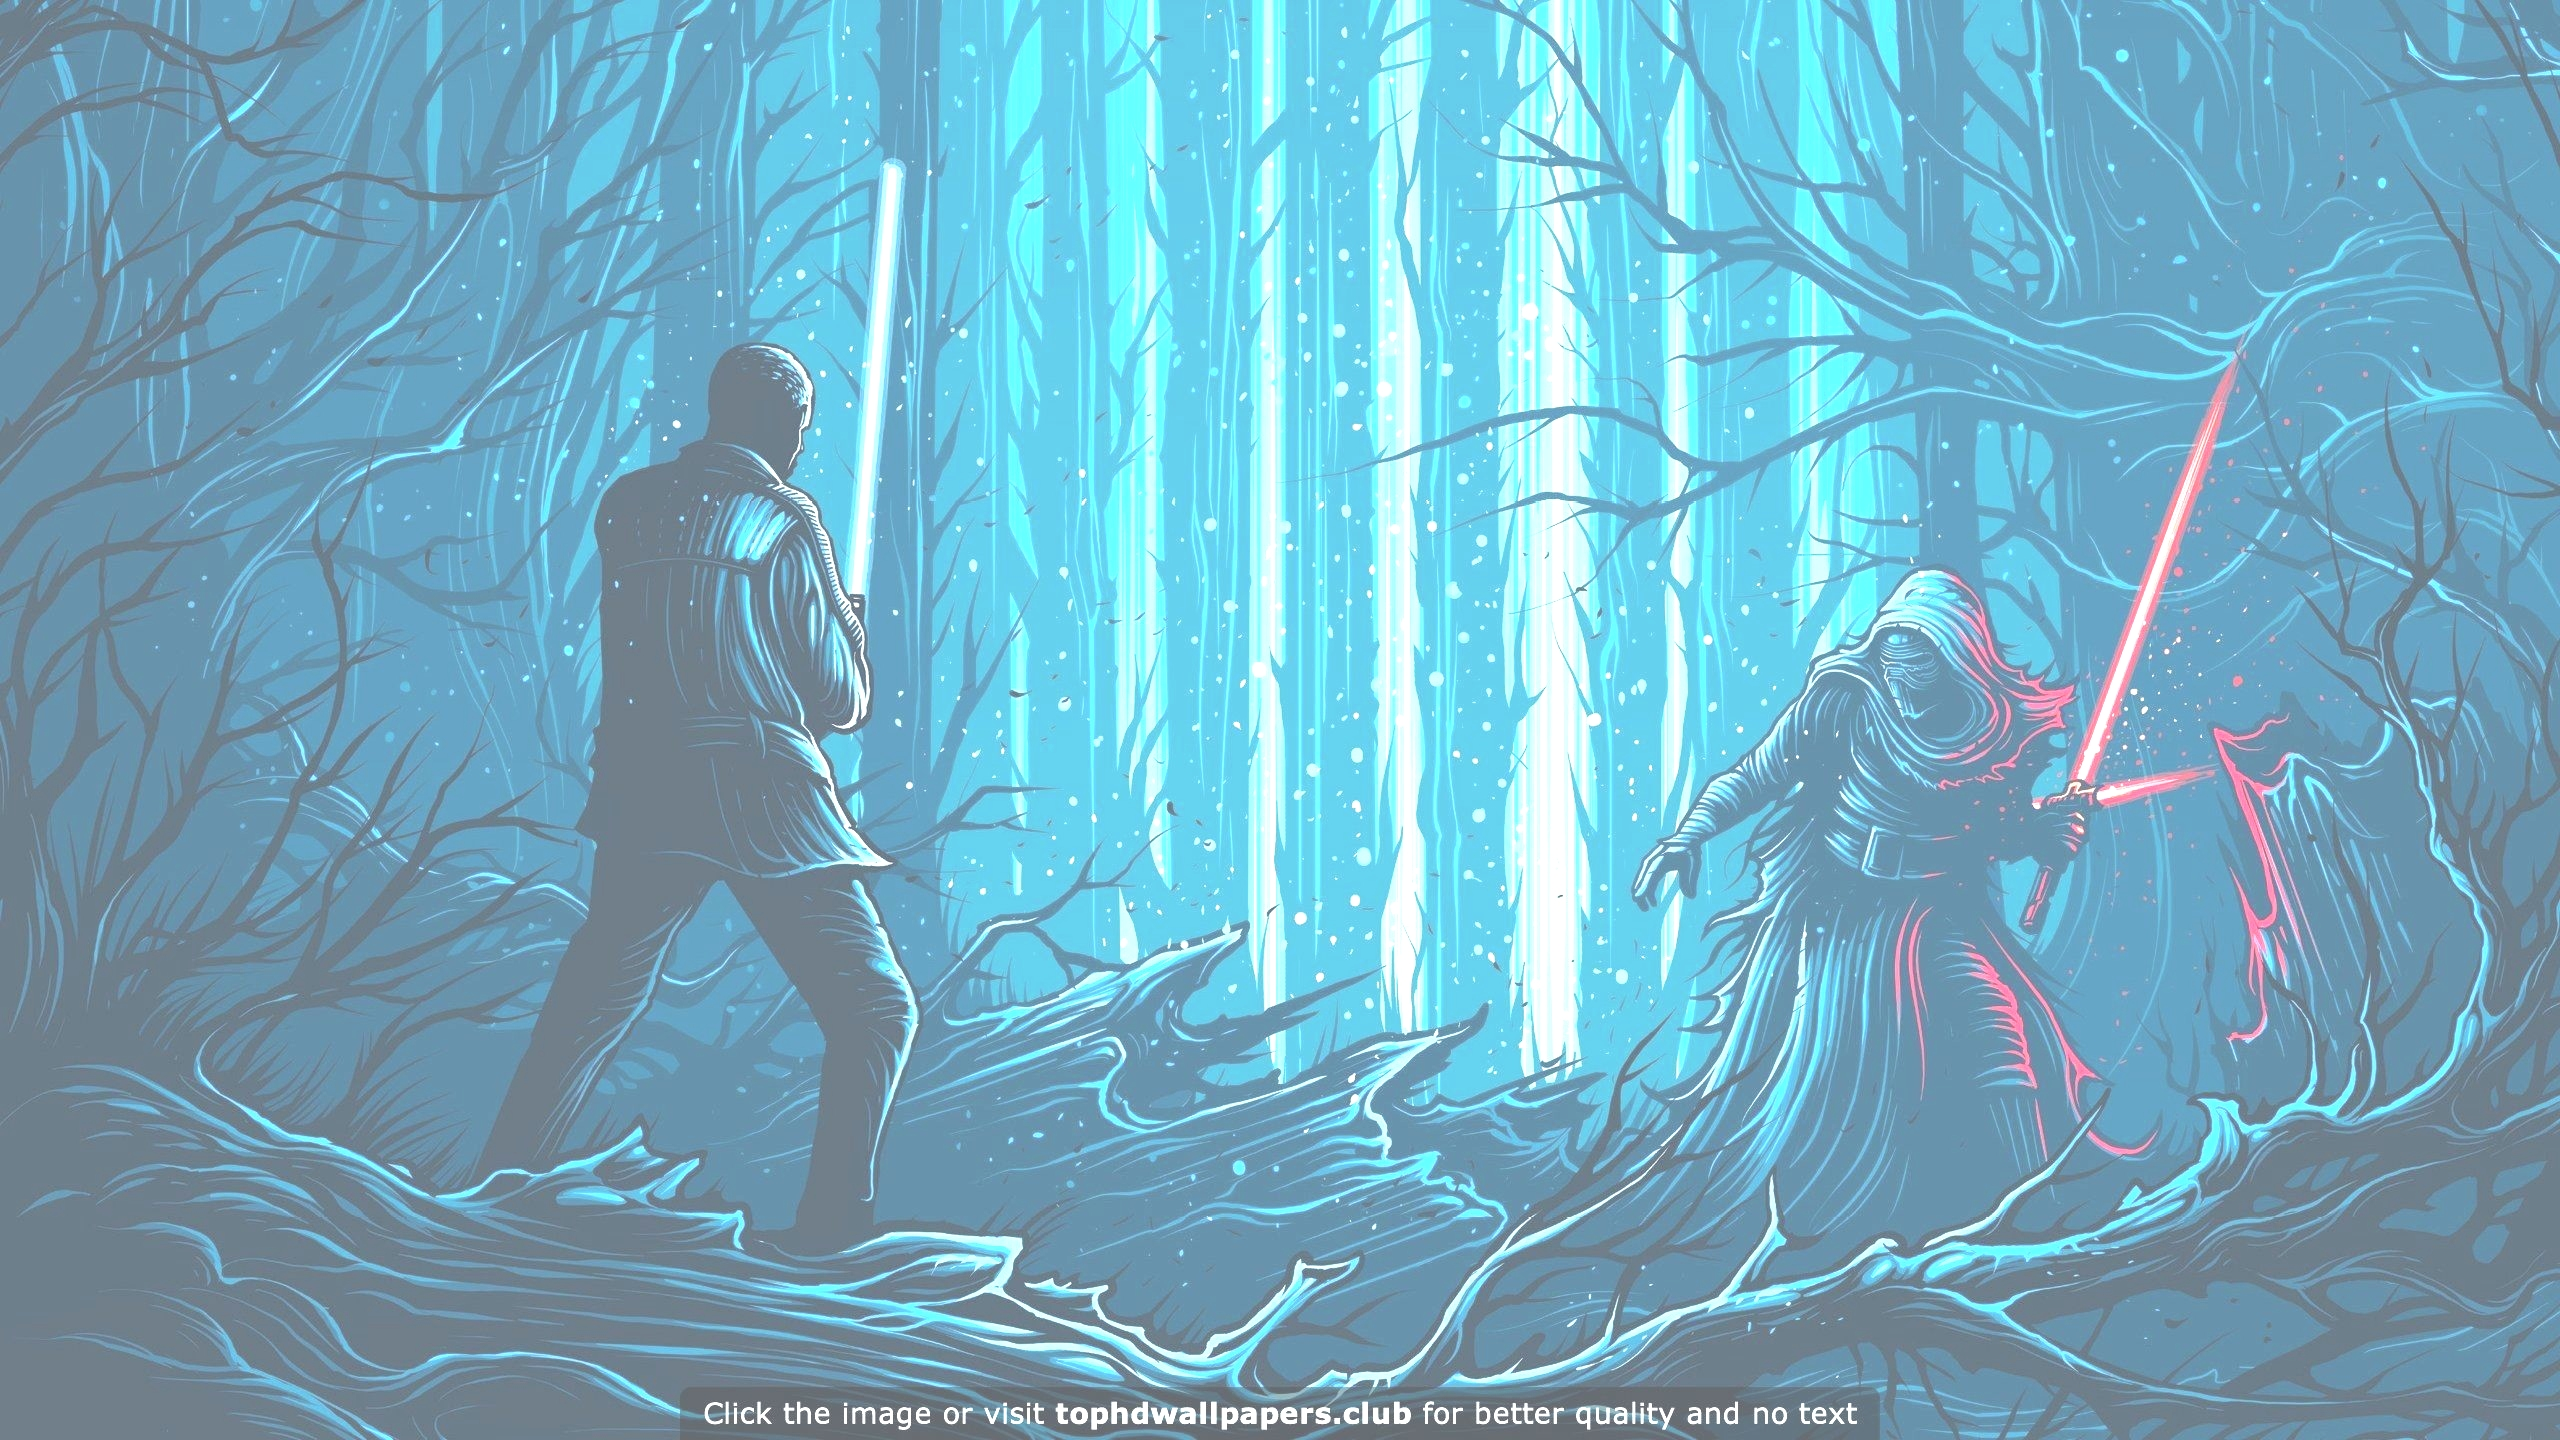
\includegraphics[width=0.5\textwidth]{report_src/brightness_high.jpeg}

\emph{Méthode appelante : Retouching.setBrightness()}

\emph{Script : brightness.rs}
\\

Ce réglage se contente d'ajouter une valeur (positive ou négative) aux trois canaux RGB de l'image. Cette valeur est fixée par la seekbar.
Les valeurs sont tronquées entre 0 et 255, par conséquent on perd de l'information dans les valeurs extrêmes de luminosité.

Cet effet n'utilise pas la luminosité existante de l'image, ainsi on peut obtenir des résultats qui sont parfois discutables, par exemple
le noir qui s'éclaircit et inversement pour le blanc. Pour pallier à ce problème, on pourrait introduire une multiplication afin de modifier
la luminosité proportionnellement à celle existante. Cependant, cette solution modifie aussi le contraste, nous avons donc choisi
de laisser l'algorithme tel quel.


\subsection{Contraste (Contrast) :}

\emph{Méthode appelante : Retouching.dynamicExtensionRGB()}

\emph{Script : dynamicExtension.rs}
\\

Ce réglage effectue une extension linéaire de dynamique. Les nouveaux extremum de l'histogramme sont définis à partir de la position de la seekbar.
La dynamique est ainsi étendue autour d'une valeur se situant au milieu des deux anciens extremum de l'histogramme*. On a donc une image uniforme lorsque
l'on règle le contraste au minimum.
\\
Le principal problème de l'extension dynamique est qu'elle ne permet pas d'augmenter le contraste à des grandes valeurs. En effet, les extremum sont vite
atteints. La solution serait de faire une transformation linéaire par morceaux.
\\

*Il serait peut-être plus juste de prendre la médiane de l'histogramme cumulé afin d'avoir une valeur qui représente mieux la "valeur moyenne" de l'image.


\subsection{Saturation (Saturation) :}





\subsection{Convolution (Blur, Sharpen, Neon) :}

    Dans cette sous-section on retrouve des effets pour flouter une image en passant par deux types différents de kernel : Gaussien et moyenneur
    (bouton "Blur"), des effets pour améliorer la netteté d'une image avec la fonction "Laplacian of gaussian" (bouton Sharpen) et des effets de 
    détection de contours (bouton "Neon") en réalisant une convolution avec des opérateurs comme Sobel, Prewitt, Kirsch ou simplement avec un kernel
    de Laplace.
    \\

    Pour cet effet nous avons implémenté 3 méthodes de convolution.

    

    \begin{itemize}
        \item Convolution classique.
        \item Convolution séparable.
        \item Produit de convolution.
    \end{itemize}

    \subsubsection*{Convolution classique}
    
        Cette méthode de convolution suit le même algorithme vu en cours, on peut l'appliquer avec des noyaux asymétriques de dimensions impaires uniquement,
        cette opération a été parallélisée grâce à l'outil "renderscript" qui parallélise le calcul par CPU multithreading/GPU. En plus dans cette méthode (et dans toutes les autres) nous avons rajouté
        des optimisations pour parcourir seulement les index nécessaires de l'image lors de la convolution. En calculant les index des centres des deux dimensions du kernel
        on peut anticiper et éviter les appels de fonction inutiles sur les bords de l'image par exemple.
        \newpage
        
        $X_{d\acute{e}but}$ et $X{fin}$ étant le premier et dernier index à parcourir dans l'axe des abscisses respectivement et
        $Y_{d\acute{e}but}$ et $Y_{fin}$ étant le premier et dernier index à parcourir dans l'axe des ordonnées respectivement.
        \[
            Kernel_{CentreX} =   \frac{Largeur_{kernel}}{2}            
        \]
        \[
            Kernel_{CentreY} =   \frac{Hauteur_{kernel}}{2}            
        \]
        \[
            X_{d\acute{e}but} = Kernel_{CentreX}      
        \]
        \[
            X_{fin} = Largeur_{image} - Kernel_{CentreX}           
        \]
        \[
            Y_{d\acute{e}but} = Kernel_{CentreY}      
        \]
        \[
            Y_{fin} = Hauteur_{image} - Kernel_{CentreY}           
        \]

        En définissant les index du début et de fin de parcours pour les deux dimensions de l'image sur le script de lancement renderscript
        comme ci-dessus on peut s'en passer de quelques appels de fonctions sur les bords de l'image et ainsi gagner du temps de calcul.

    \subsubsection*{Convolution séparable}

        Pour la convolution classique avec un kernel de taille $N*M$ on doit faire $N*M$ multiplications pour chaque échantillon,
        cependant si le kernel est séparable on peut passer à $N+M$ opérations.
        \\

        Or afin d'optimiser le calcul de la convolution sur des filtres séparables comme le filtre gaussien et moyenneur nous avons implémenté une
        méthode de convolution séparable.
        
        \begin{figure}[!h]
            \centering
            \begin{subfigure}[b]{1\textwidth}
                \centering
                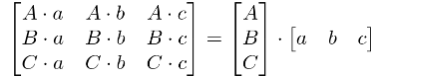
\includegraphics[width=0.5\textwidth]{report_src/separableConv1.png}
            \end{subfigure}
        \end{figure}

        Un kernel est séparable quand sa matrice des poids peut être représentée par le produit de deux vecteurs.
        \\

        Ce calcul est réalisé en faisant deux convolutions unidimensionnelles successives (en X et en Y) sur l'image d'origine en stockant le résultat dans une image intermédiaire.
        La propriété d'associativité de la convolution rend ce calcul possible.

        \[
            x * (N * N)  \iff (x * N) * N
        \]

        La limite de cette méthode c'est que l'on doit passer par une image partielle pour la réalisation du calcul en
        utilisant plus de mémoire que pour une convolution classique.



    \subsubsection*{Produit de convolution}

        Cette méthode prend en paramètre deux kernels de même taille et réalise deux convolutions avec chaque kernel et ensuite calcule le produit des deux.
        Vu que ces deux convolutions sont indépendantes l'une de l'autre on peut se permettre de les réaliser au même temps dans le script et de faire l'addition
        des valeurs absolues résultantes des deux accumulateurs. Cette méthode est utilisé notamment pour faire des convolutions avec les opérateurs de Sobel, Kirsch, Prewitt.


    \subsubsection{Flou gaussien et moyenneur (Blur) : }

        \begin{figure}[!h]
            \centering
            \begin{subfigure}[b]{0.4\textwidth}
                \includegraphics[width=1\textwidth]{report_src/picOrg.jpeg}
            \end{subfigure}
            \begin{subfigure}[b]{0.4\textwidth}
                
\includegraphics[width=1\textwidth]{report_src/blur.jpeg}
            \end{subfigure}
            \caption{Image originale et image avec flou gaussien
                    Méthode appelante }
        \end{figure}





        
